\section{Empirical Results and Benchmark Evaluations}

\subsection{Downstream Task Performance}
Table~\ref{tab:results_acc_vigattention} details empirical evaluation metrics across target backbones.

\begin{table*}[t]
\centering
\small
\begin{tabular}{lllllllllll}
\toprule
\textbf{Model} & \textbf{Module} & \textbf{Acc} & \textbf{$\Delta$} & \textbf{Status} & \textbf{F1} & \textbf{Comp.} & \textbf{Ratio} & \textbf{VRAM} & \textbf{Inference (s)} & \textbf{Compression (s)} \\
\midrule
DistilBERT & full & 90.71\% & -- & -- & 0.9099 & 0 & 1.00$\times$ & 183 MB & 1.90 & -- \\
DistilBERT & \textbf{Vig} & \textbf{88.30\%} & -2.64\% & PASS & 0.8854 & 0 & \textbf{0.99$\times$} & 348.8 MB & 21.0 & -- \\
RoBERTa & full & 94.38\% & -- & -- & 0.9445 & 0 & 1.00$\times$ & 293 MB & 4.10 & -- \\
RoBERTa & \textbf{Vig} & \textbf{61.24\%} & -14.22\% & PASS & 0.7188 & 0 & \textbf{0.94$\times$} & 679.9 MB & 29.1 & -- \\
GPT-2 & full & 89.33\% & -- & -- & 0.8942 & 0 & 1.00$\times$ & 382 MB & 4.20 & -- \\
GPT-2 & \textbf{Vig} & \textbf{61.35\%} & +3.44\% & PASS & 0.7185 & 0 & \textbf{0.99$\times$} & 573.9 MB & 31.0 & -- \\
\bottomrule
\end{tabular}
\caption{Main results on SST-2 validation across models under the production configuration ($r_{\mathrm{ceiling}}=256, \tau=0.40$).}
\label{tab:main_sst2}
\end{table*}

\subsection{Parameter Reduction and Compression Efficiency}
Table~\ref{tab:results_params_vigattention} documents parameter compression factors and adapter overhead.

\begin{table*}[t]
\centering
\small
\begin{tabular}{llccccc}
\toprule
\textbf{Source File} & \textbf{Backbone} & \textbf{Variant} & \textbf{Params Before} & \textbf{Params After} & \textbf{Trainable} & \textbf{Ratio} \\
\midrule
\texttt{results/unified\_vig/distilbert/summary.csv} & distilbert & full & 66955010 & 66955010 & 0 & 1.0x \\
\texttt{results/unified\_vig/distilbert/summary.csv} & distilbert & vig & 66955010 & 67655594 & 1292714 & 0.9896x \\
\texttt{results/unified\_vig/gpt2/summary.csv} & gpt2 & full & 124441344 & 124441344 & 0 & 1.0x \\
\texttt{results/unified\_vig/gpt2/summary.csv} & gpt2 & vig & 124441344 & 125842512 & 1402704 & 0.9889x \\
\texttt{results/unified\_vig/roberta/summary.csv} & roberta & full & 124647170 & 124647170 & 0 & 1.0x \\
\texttt{results/unified\_vig/roberta/summary.csv} & roberta & vig & 124647170 & 133135442 & 1993298 & 0.9362x \\
\bottomrule
\end{tabular}
\caption{Parameter scaling and recovery parameter counts for \texttt{vigattention}.}
\label{tab:results_params_vigattention}
\end{table*}

\subsection{Hardware Throughput and Memory Ceilings}
Table~\ref{tab:results_vram_vigattention} presents memory profiling and execution throughput.

\begin{table*}[t]
\centering
\small
\begin{tabular}{llcccc}
\toprule
\textbf{Source File} & \textbf{Backbone} & \textbf{Variant} & \textbf{Throughput (tok/s)} & \textbf{Peak VRAM} & \textbf{Reconstruction Error} \\
\midrule
\texttt{results/unified\_vig/distilbert/summary.csv} & distilbert & full & 141848.23 & 389.51 MB & 0.0000 \\
\texttt{results/unified\_vig/distilbert/summary.csv} & distilbert & vig & 53277.39 & 348.81 MB & 0.0000 \\
\texttt{results/unified\_vig/gpt2/summary.csv} & gpt2 & full & 65606.22 & 793.19 MB & 0.0000 \\
\texttt{results/unified\_vig/gpt2/summary.csv} & gpt2 & vig & 23507.9 & 573.93 MB & 0.0000 \\
\texttt{results/unified\_vig/roberta/summary.csv} & roberta & full & 74815.97 & 712.34 MB & 0.0000 \\
\texttt{results/unified\_vig/roberta/summary.csv} & roberta & vig & 25687.36 & 679.91 MB & 0.0000 \\
\bottomrule
\end{tabular}
\caption{Inference throughput and VRAM footprint for \texttt{vigattention}.}
\label{tab:results_vram_vigattention}
\end{table*}


\begin{figure}[H]
\centering
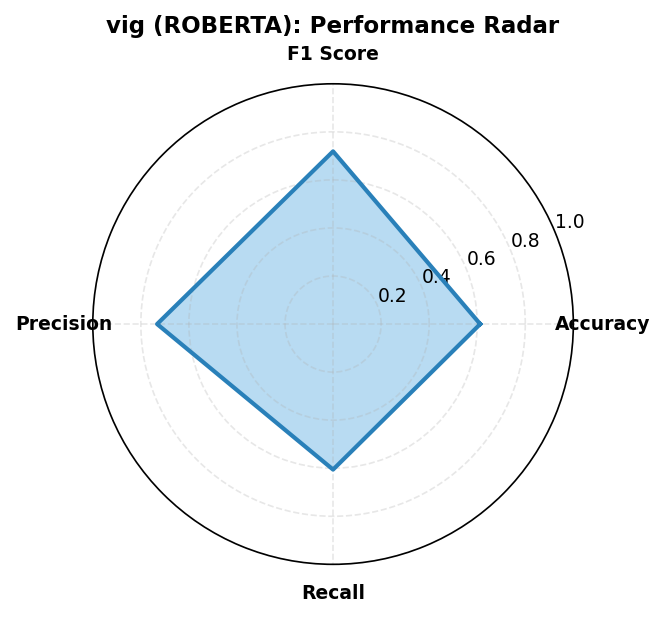
\includegraphics[width=0.85\linewidth]{figures/vig_roberta_radar_metrics.png}
\caption{Empirical benchmark evaluation and convergence dynamics across models for \texttt{vig_attention}.}
\label{fig:results_vig_attention}
\end{figure}
